\textit{Objet ? Objet-relationnel ou relationnel pur ? C'est cette question qui est traitée en premier ici. Dans une seconde partie l'utilité des ORM est expliquée, puis les templates de l'application seront présentés.}

\section{Une histoire de paradigmes}
\subsection{Le paradigme objet}

Le modèle objet pour le stockage des données présente les mêmes avantages que pour la programmation orienté objet, à savoir une grande capacité d'abstraction, de factorisation et de maintenance. Malheureusement ce paradigme n'est que peu implémenté par les SGBD (O2, db4o, ObjectStore) ce qui nuit grandement à la portabilité d'une application basé sur ce paradigme.

\subsection{Le paradigme objet-relationnel}

De nombreux SGBD tels que ORACLE offrent un paradigme hybride entre l'objet et le relationnel, l'objet-relationnel.
Ce paradigme est standardisé par la norme SQL3 cependant celle-ci n'est jamais implémentée dans sa globalité ce qui pose à nouveau un problème de portabilité (un script SQL pour ORACLE ne s'exécutera pas sur PostgreSQL et vice-versa).

\subsubsection{Schéma objet-relationnel}

Voici le script ORACLE de création des types et tables pour notre application, utilisant des aspect objet-relationnel.
\lstinputlisting[language=sql]{./sources/schema_objet_relationnel.sql}

\subsection{Le paradigme relationnel pur}

La vision historique des bases de données est le relationnel pur, il offre des performances reconnus. En revanche, son utilisation peut poser problème lors d'une modélisation objet de l'application. If faut alors créer un nouveau schéma pour la base de données, et développer des procédures de stockage pour gérer la persistance des objets.

\subsubsection{Schéma relationnel}

Le schéma relationnel pur présenté ci-dessous permet la persistance des objets nécessaire à notre application. D'après le diagramme UML de classe, nous avons ajouté une table des synonymes et une table d'associations.

\begin{description}
\item[TERME](\underline{lib\_terme})
\item[CONCEPT](\underline{terme\_vedette}\up{\#}, concept\_general\up{\#})
\item[SYNONYME](\underline{terme\up{\#}, concept\up{\#}})
\item[ASSOCIATION](\underline{concept1\up{\#}, concept2\up{\#}})
\end{description}

\section{ORM}

	\subsection{Qu'est qu'un ORM?}
    Un ORM ou \emph{mapping objet-relationnel} (en anglais \emph{object-relational mapping}) est un outil informatique qui donne l'illusion d'une base de données orientée objet à partir d'une base de données relationnelle en servant d'interface entre celle-ci et le code de l'application.
   
	\subsection{Pourquoi?}
    Nous avons vu que les systèmes de gestion de base de données orientées objet sont actuellement peu nombreuses, que la norme SQL3 n'est que partiellement implémentée, notamment sur le SGBD Postgresql que nous avons décidé d'utiliser.
    
En revanche, cette méthode d'abstraction présente le désavantage de générer un schéma différents de la vision objet avec laquelle est modélisée l'application. Il peut parfois être nécessaire d'intervenir directement dans la base de données (développement de TRIGGERS, dump SQL, \ldots), ce qui nécessitera un effort supplémentaire de d'analyse et de compréhension.

\section{Décisions}

\subsection{Postgresql}

Initialement, nous avions choisi de travailler avec Postpresql pour plusieurs raisons :
\begin{itemize}
\item découvrir l'objet relationnel sur un nouveau système (autre qu'ORACLE),
\item travailler avec un logiciel libre,
\item respectueux des standards SQL,
\item et précurseur aux débuts de l'objet-relationnel (premier SQL à intégrer des aspects objet).
\end{itemize}

\subsection{Framework \& ORM}

Nous avons choisi de travailler à l'aide du framework Symfony (version 2), intégrant l'ORM Doctrine (version 2). Ces outils seront présentés dans la partie suivante.

Les raisons qui nous ont poussé à faire le choix de développer l'application à l'aide d'un ORM sont les suivantes :
\begin{itemize}
\item nous avons pris conscience que l'application à développer ne nécessitait pas la vision objet-relationnel,
\item nous tenions à travailler dans un environnement libre en utilisant Postgresql, mais aujourd'hui il ne fournit pas autant de fonctions orientées objet,
\item nous souhaitions travailler avec des technologies matures,
\item nous souhaitions découvrir la mise en place d'une application à l'aide d'un ORM.
\end{itemize}
	
	
\section{Templates et formulaires}

\subsubsection{Accueil}

La page d'accueil de l'application \emph{Thésaurus Rex} est composée d'un court texte de bienvenue. La partie gauche est composée du logo, d'un champs de recherche, et de deux liens d'accès aux parties de l'application : gestion des concepts et gestion des termes. Ce panel est visible sur toutes les vues.
\begin{figure}[H]
\begin{center}
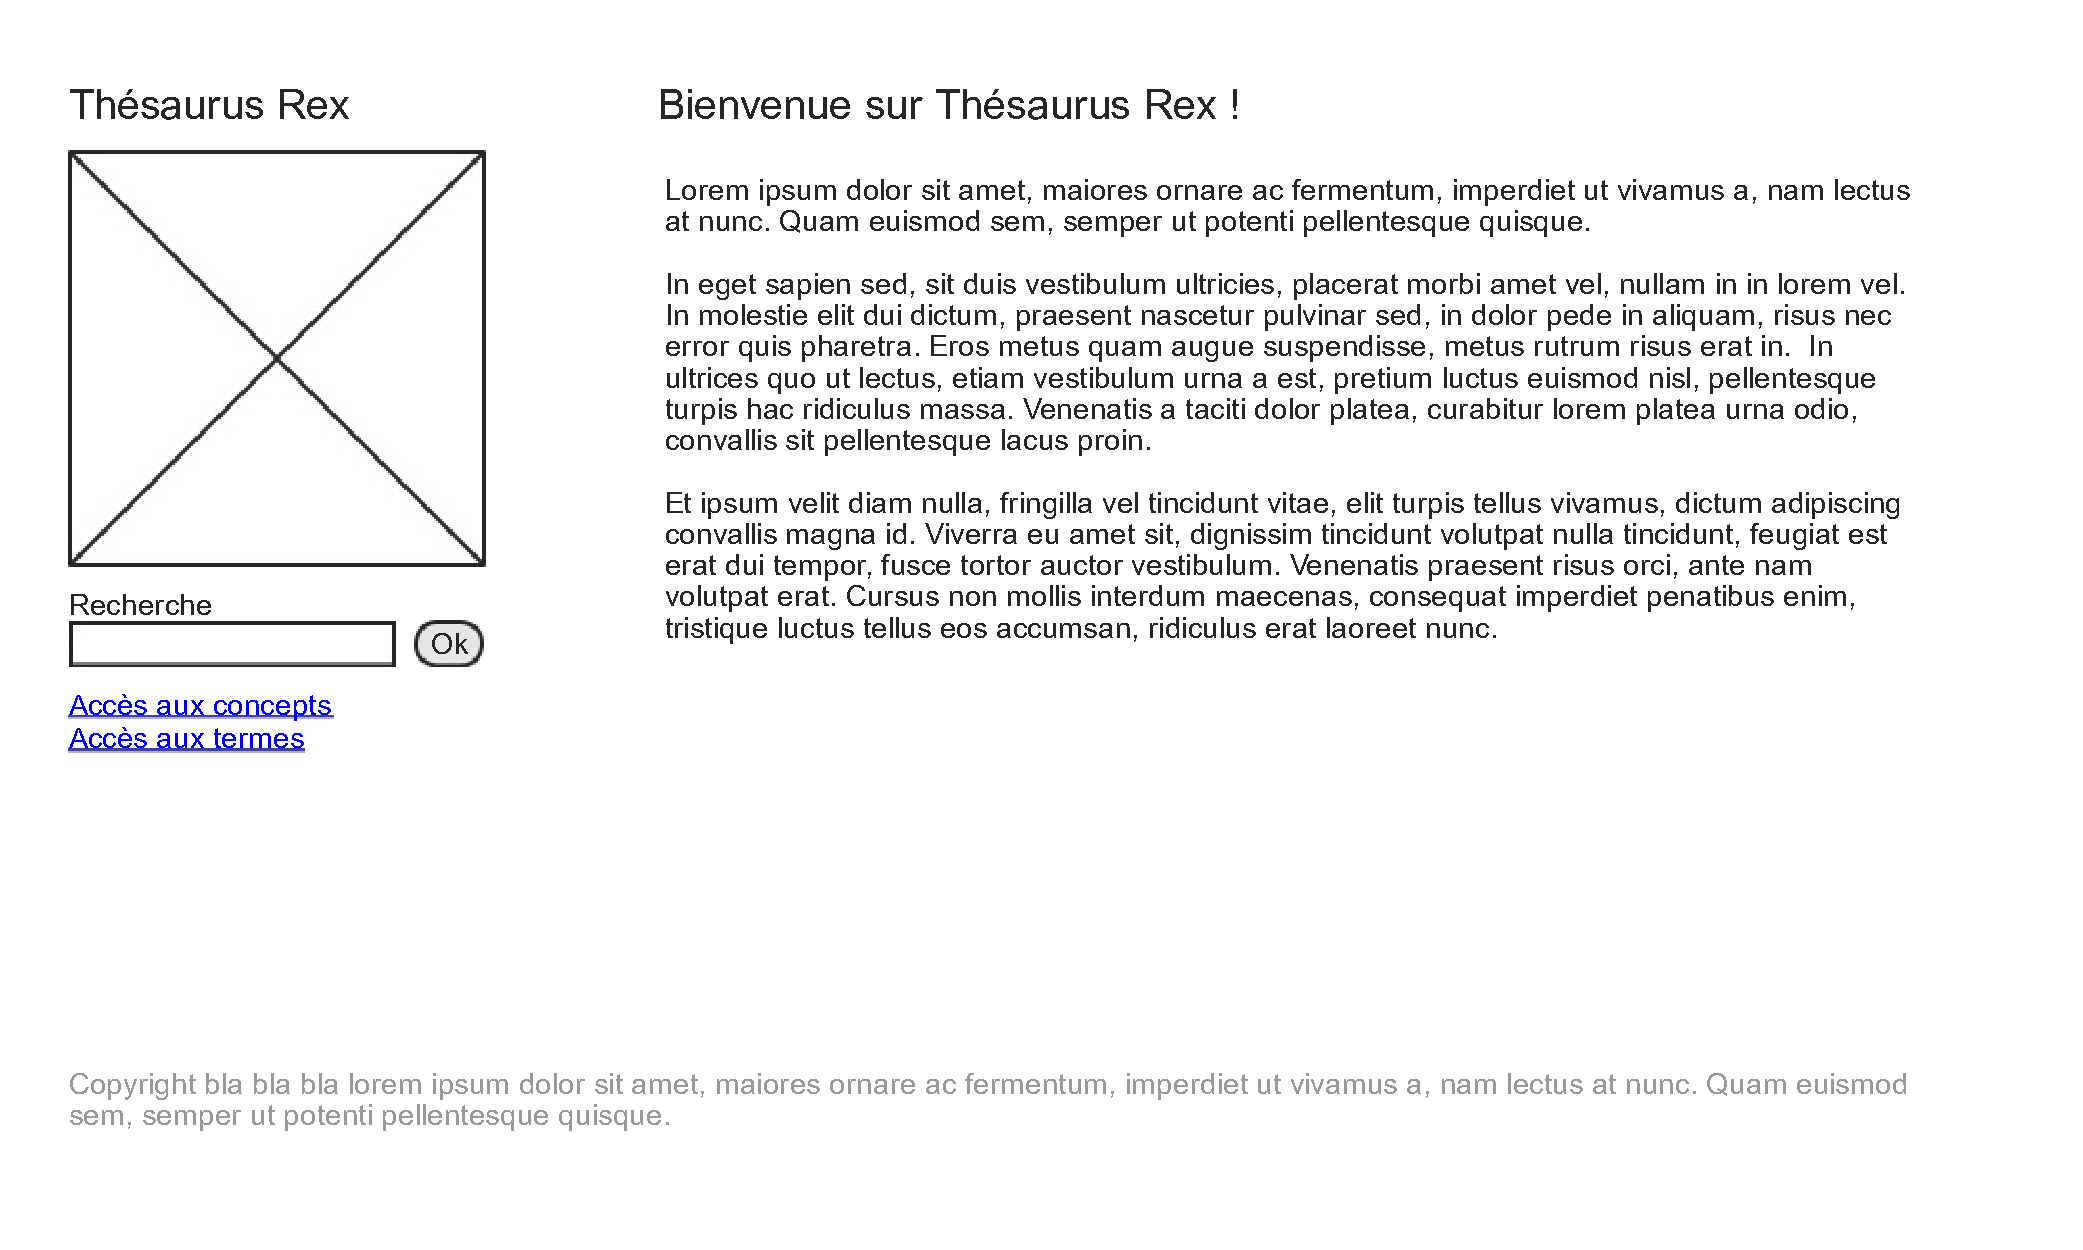
\includegraphics[width=\textwidth]{files/template_accueil}
\end{center}
\caption{Template de la page d'accueil de Thésaurus Rex.}
\end{figure}

\subsubsection{Vue hiérarchique des concepts}

La vue hiérarchique permet de visualiser l'ensemble des concepts sous la forme d'arbre en affichant le terme vedette de chaque concept. \emph{TG} signifie \emph{Terme Général},  il s'agit des racines de la hiérarchie (ils ne possèdent pas de concept général). \emph{TS} signifie \emph{Terme spécifique}, il s'agit des concepts possédant un terme général.
\begin{figure}[H]
\begin{center}
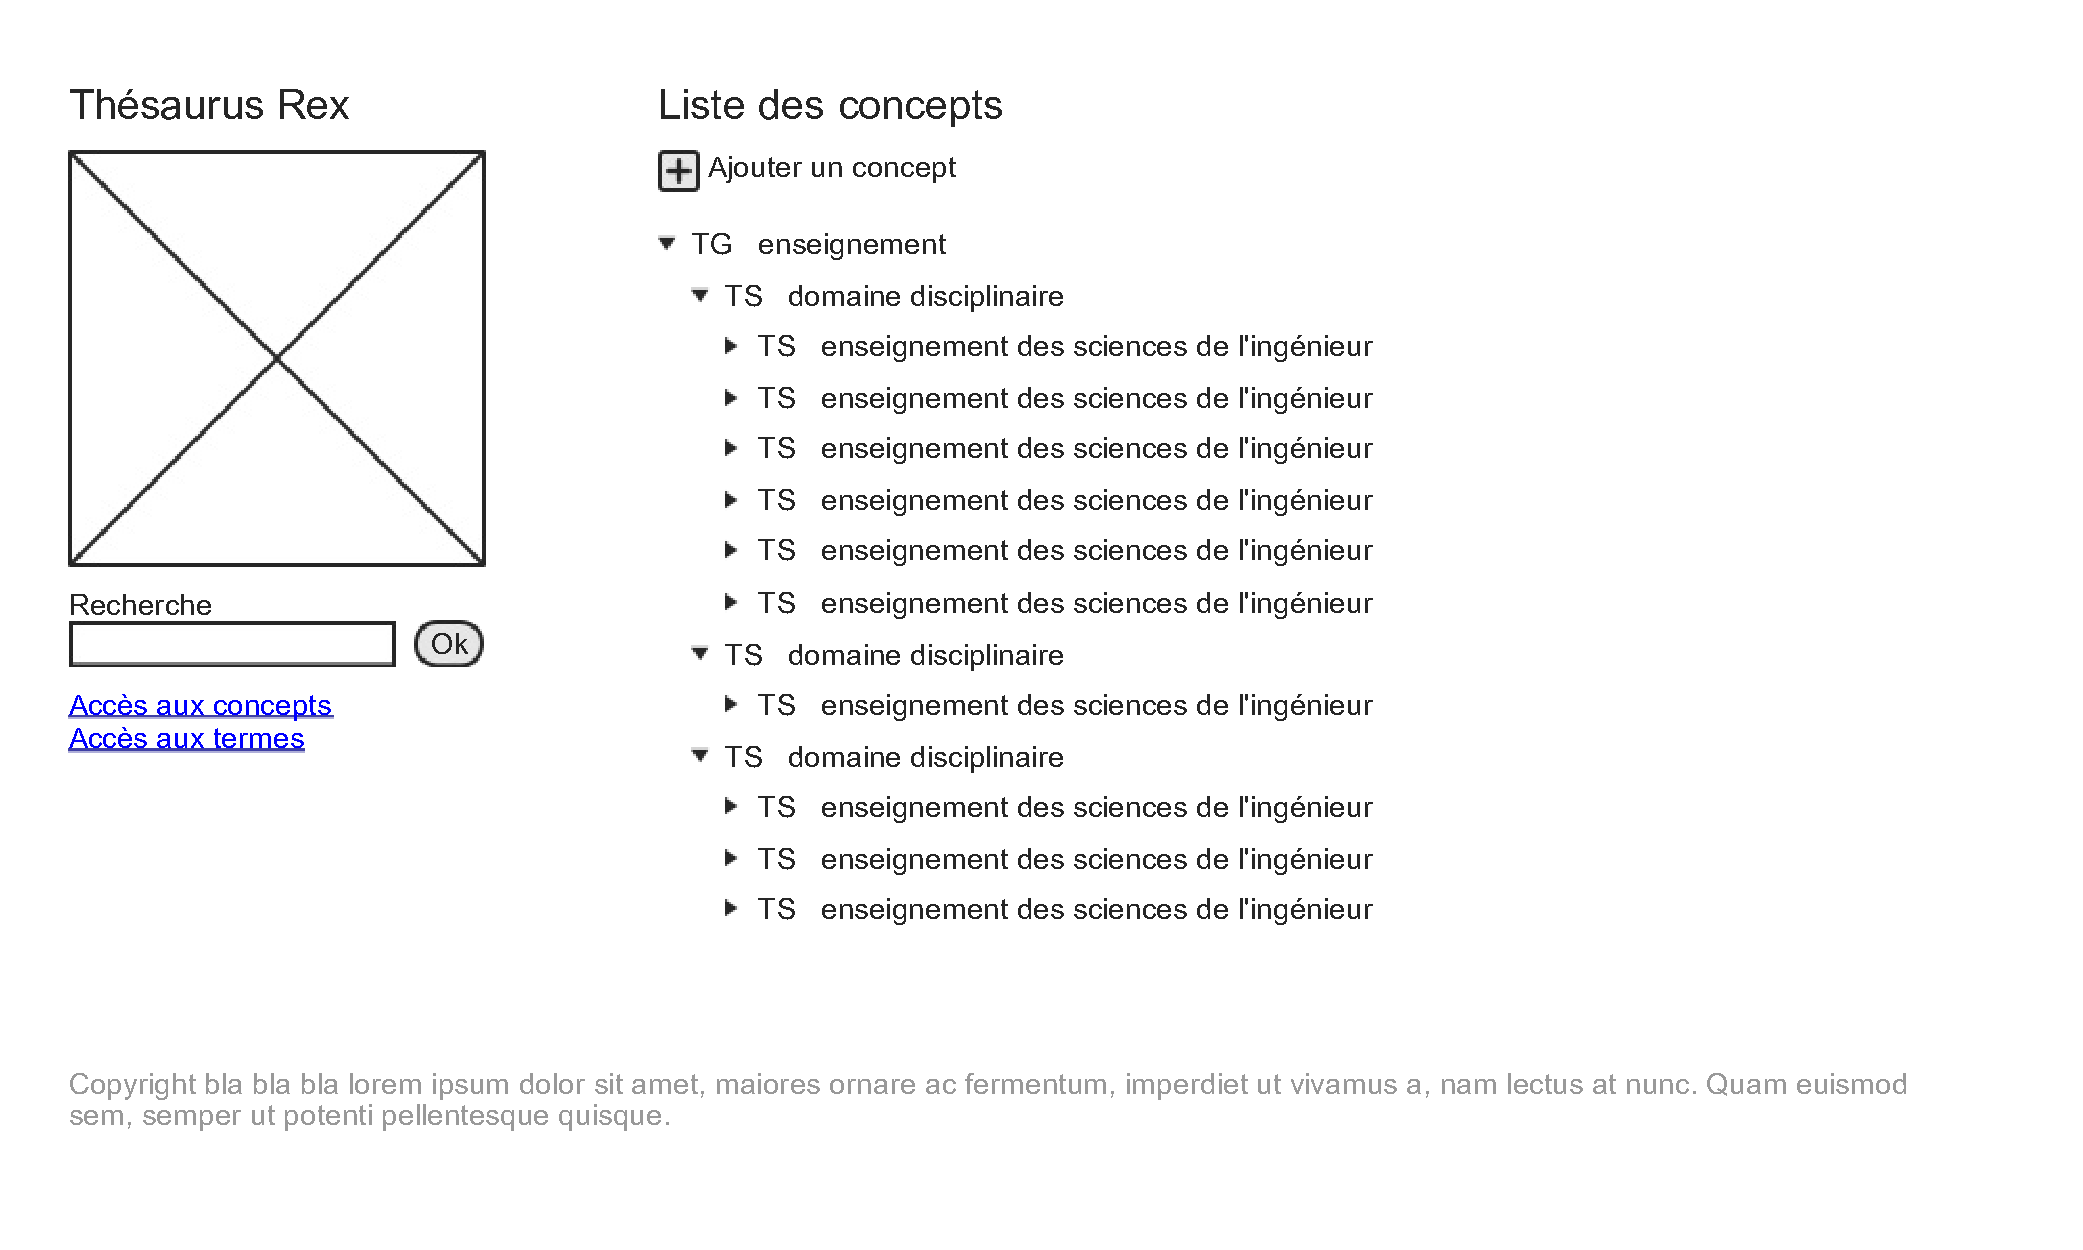
\includegraphics[width=\textwidth]{files/template_concepts}
\end{center}
\caption{Template de la vue hiérarchique des concepts.}
\end{figure}

\subsubsection{Visualisation d'un concept}

Lors du clique sur un concept à partir de la vue hiérarchique, le concept est affiché avec son environnement sémantique direct :
\begin{itemize}
\item son concept générique,
\item ses concepts spécifiques,
\item ses concepts associés,
\item ses termes synonymes.
\end{itemize}

Cette vue permet une navigation rapide dans la hiérarchie grâce à la multitude de liens.
\begin{figure}[H]
\begin{center}
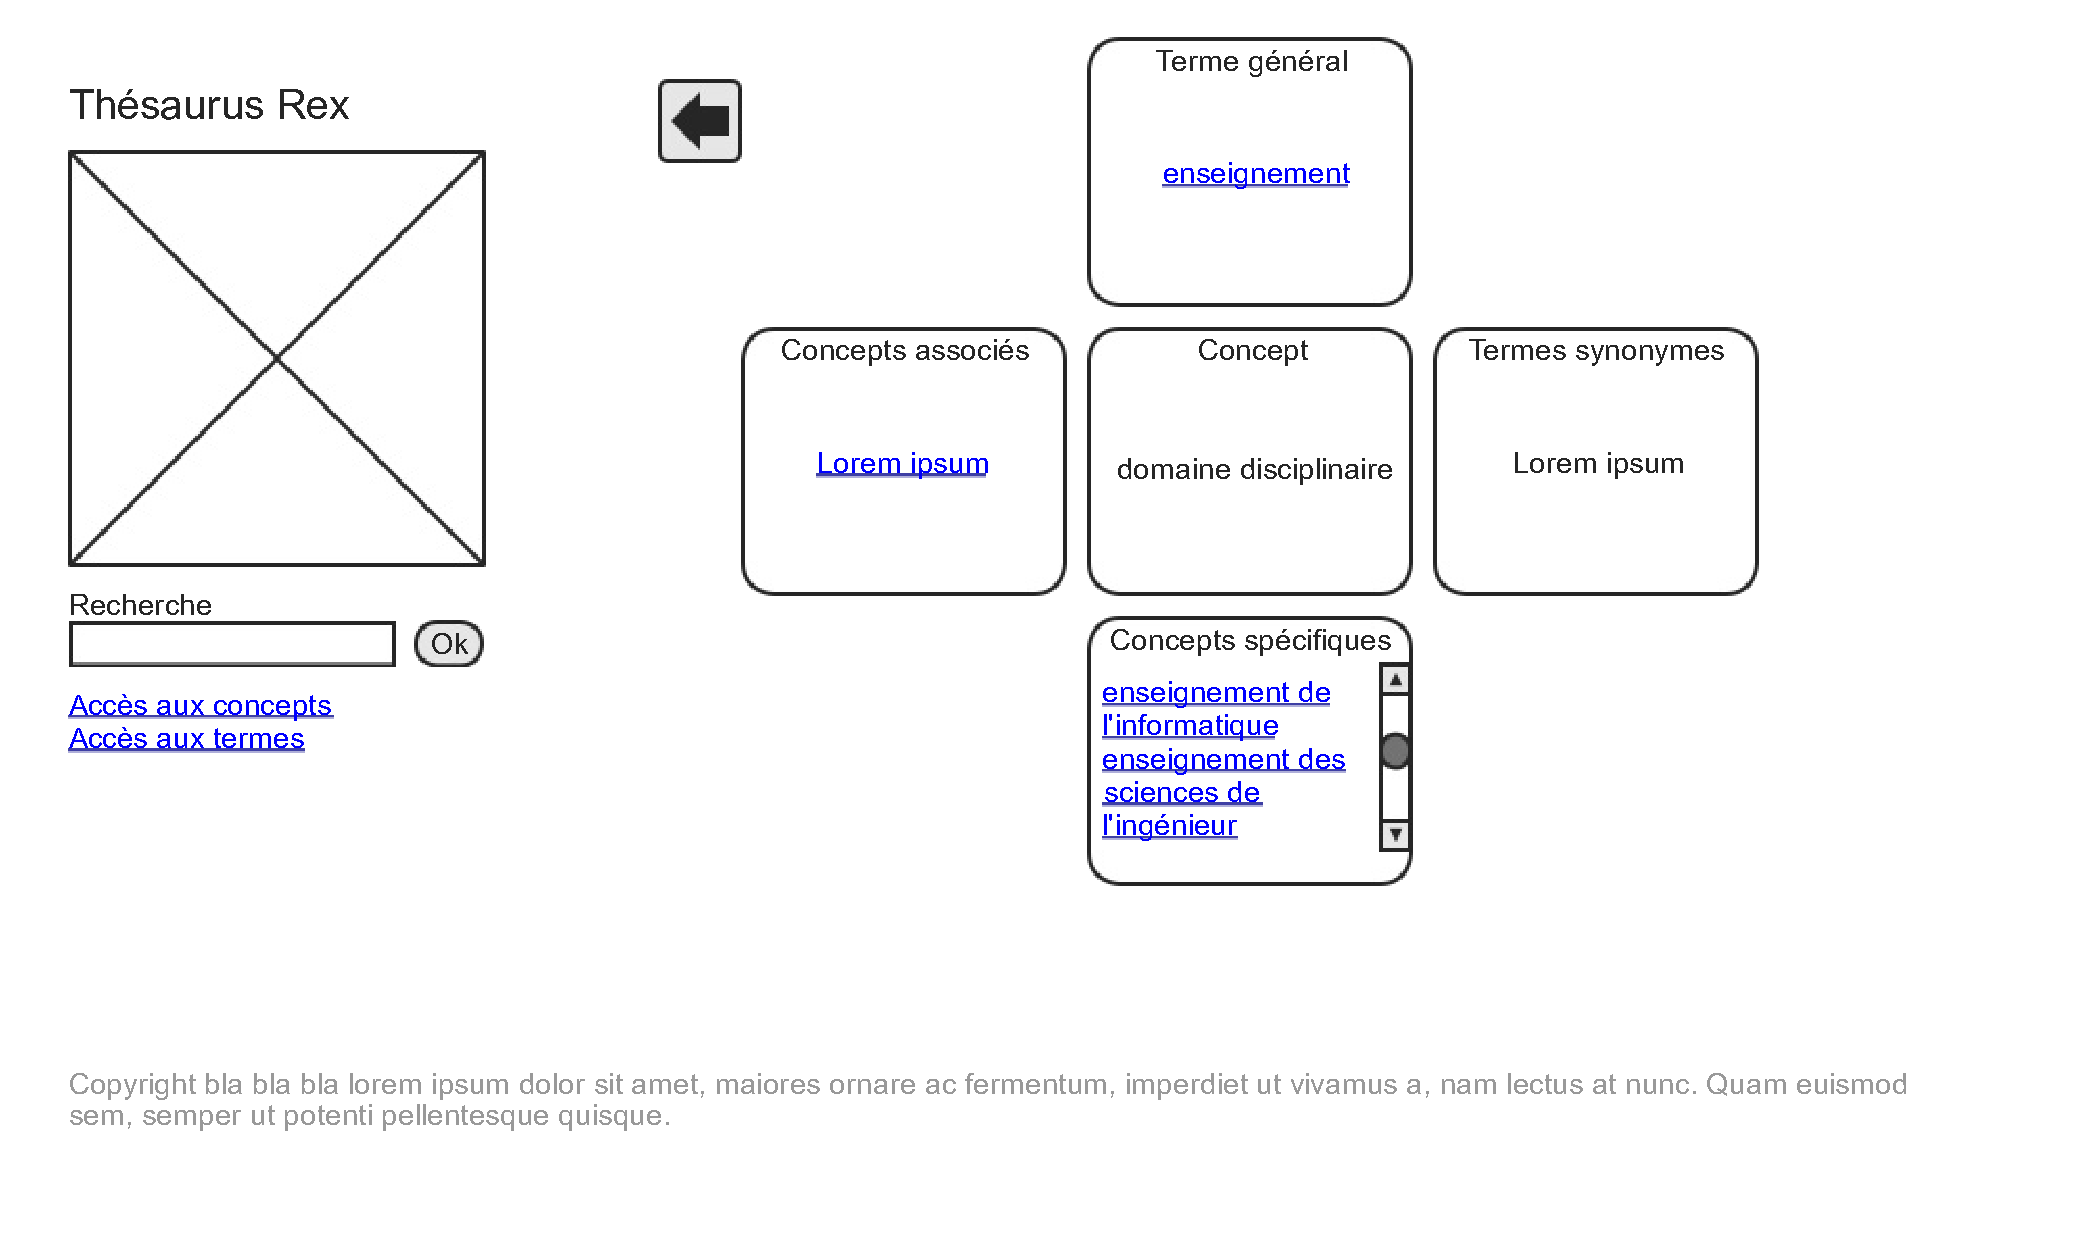
\includegraphics[width=\textwidth]{files/template_concept}
\end{center}
\caption{Template d'affichage d'un concept.}
\end{figure}

\subsubsection{Ajout / Édition d'un concept}

L'ajout et l'édition d'un concept se fait à l'aide des formulaires ci-après.
\begin{figure}[H]
\begin{center}
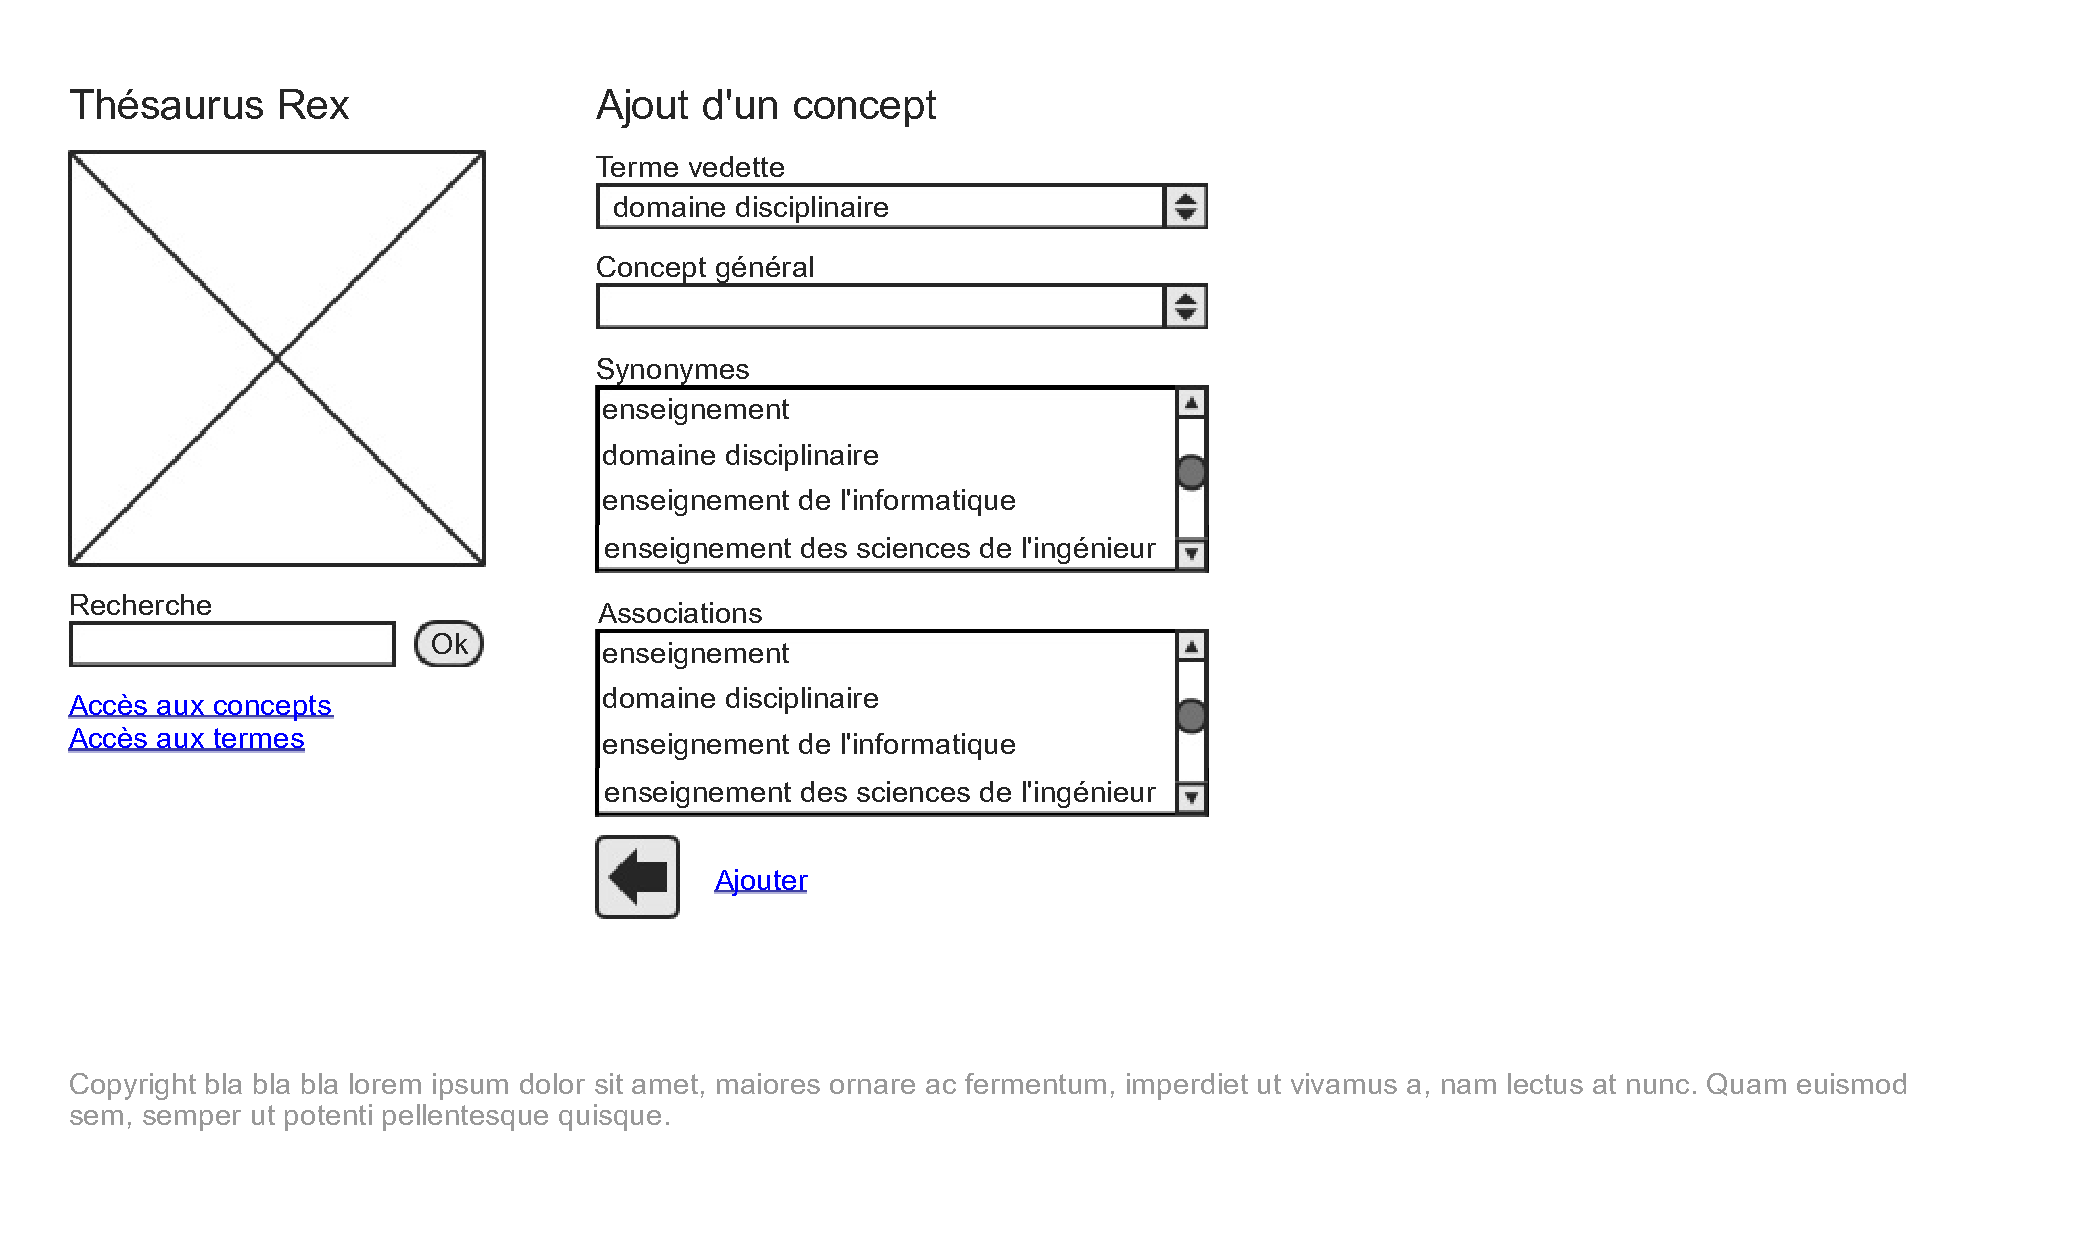
\includegraphics[width=\textwidth]{files/template_concept_add}
\end{center}
\caption{Template du formulaire d'ajout d'un concept.}
\end{figure}
\begin{figure}[H]
\begin{center}
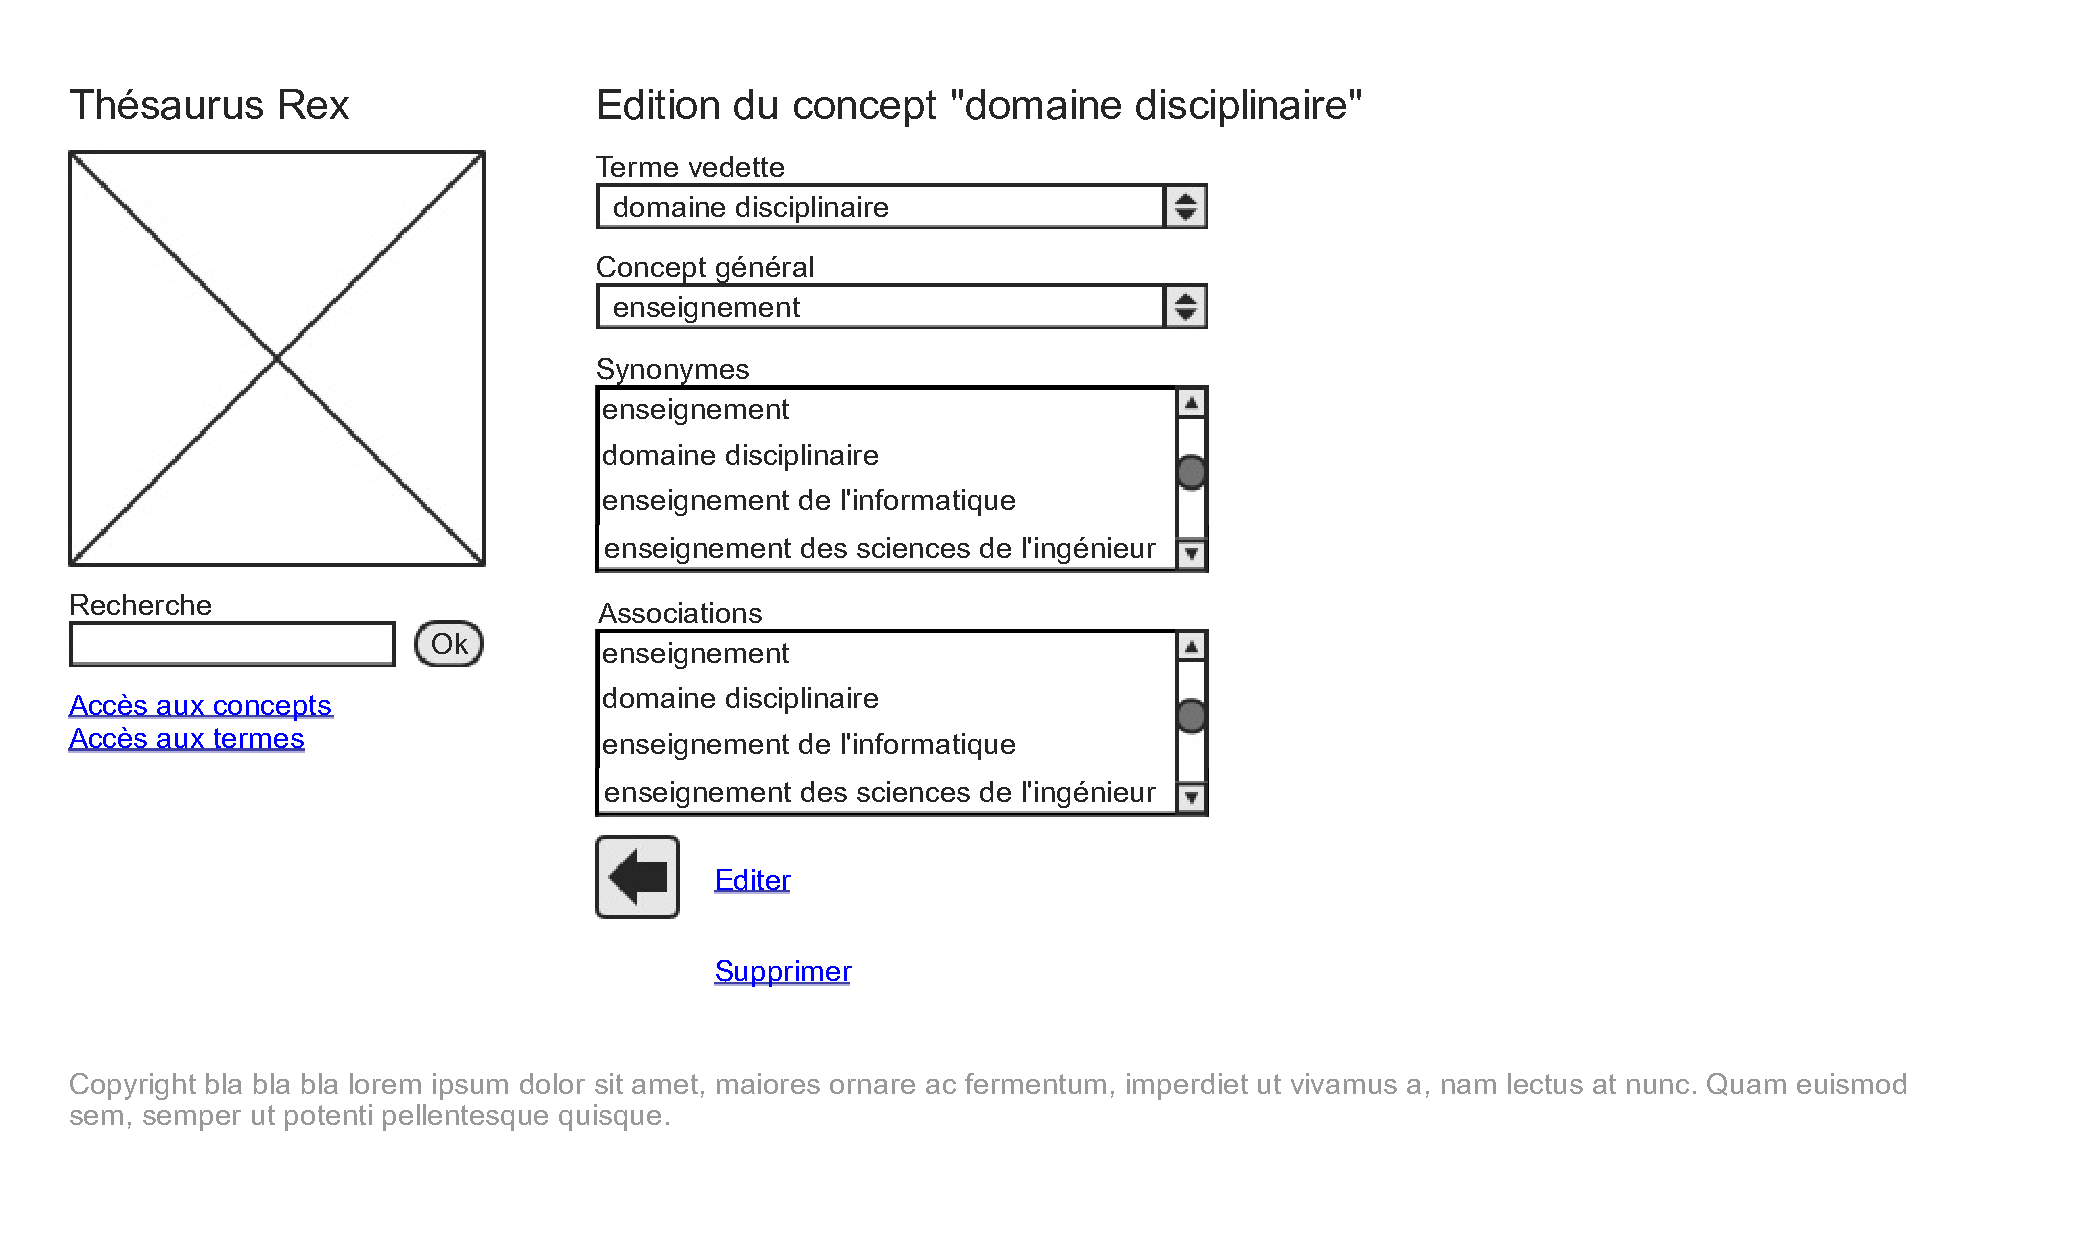
\includegraphics[width=\textwidth]{files/template_concept_edit}
\end{center}
\caption{Template du formulaire d’édition d'un concept.}
\end{figure}

\subsubsection{Liste des termes}

L'ensemble des termes peuvent être visualisés sous la forme d'une liste.
\begin{figure}[H]
\begin{center}
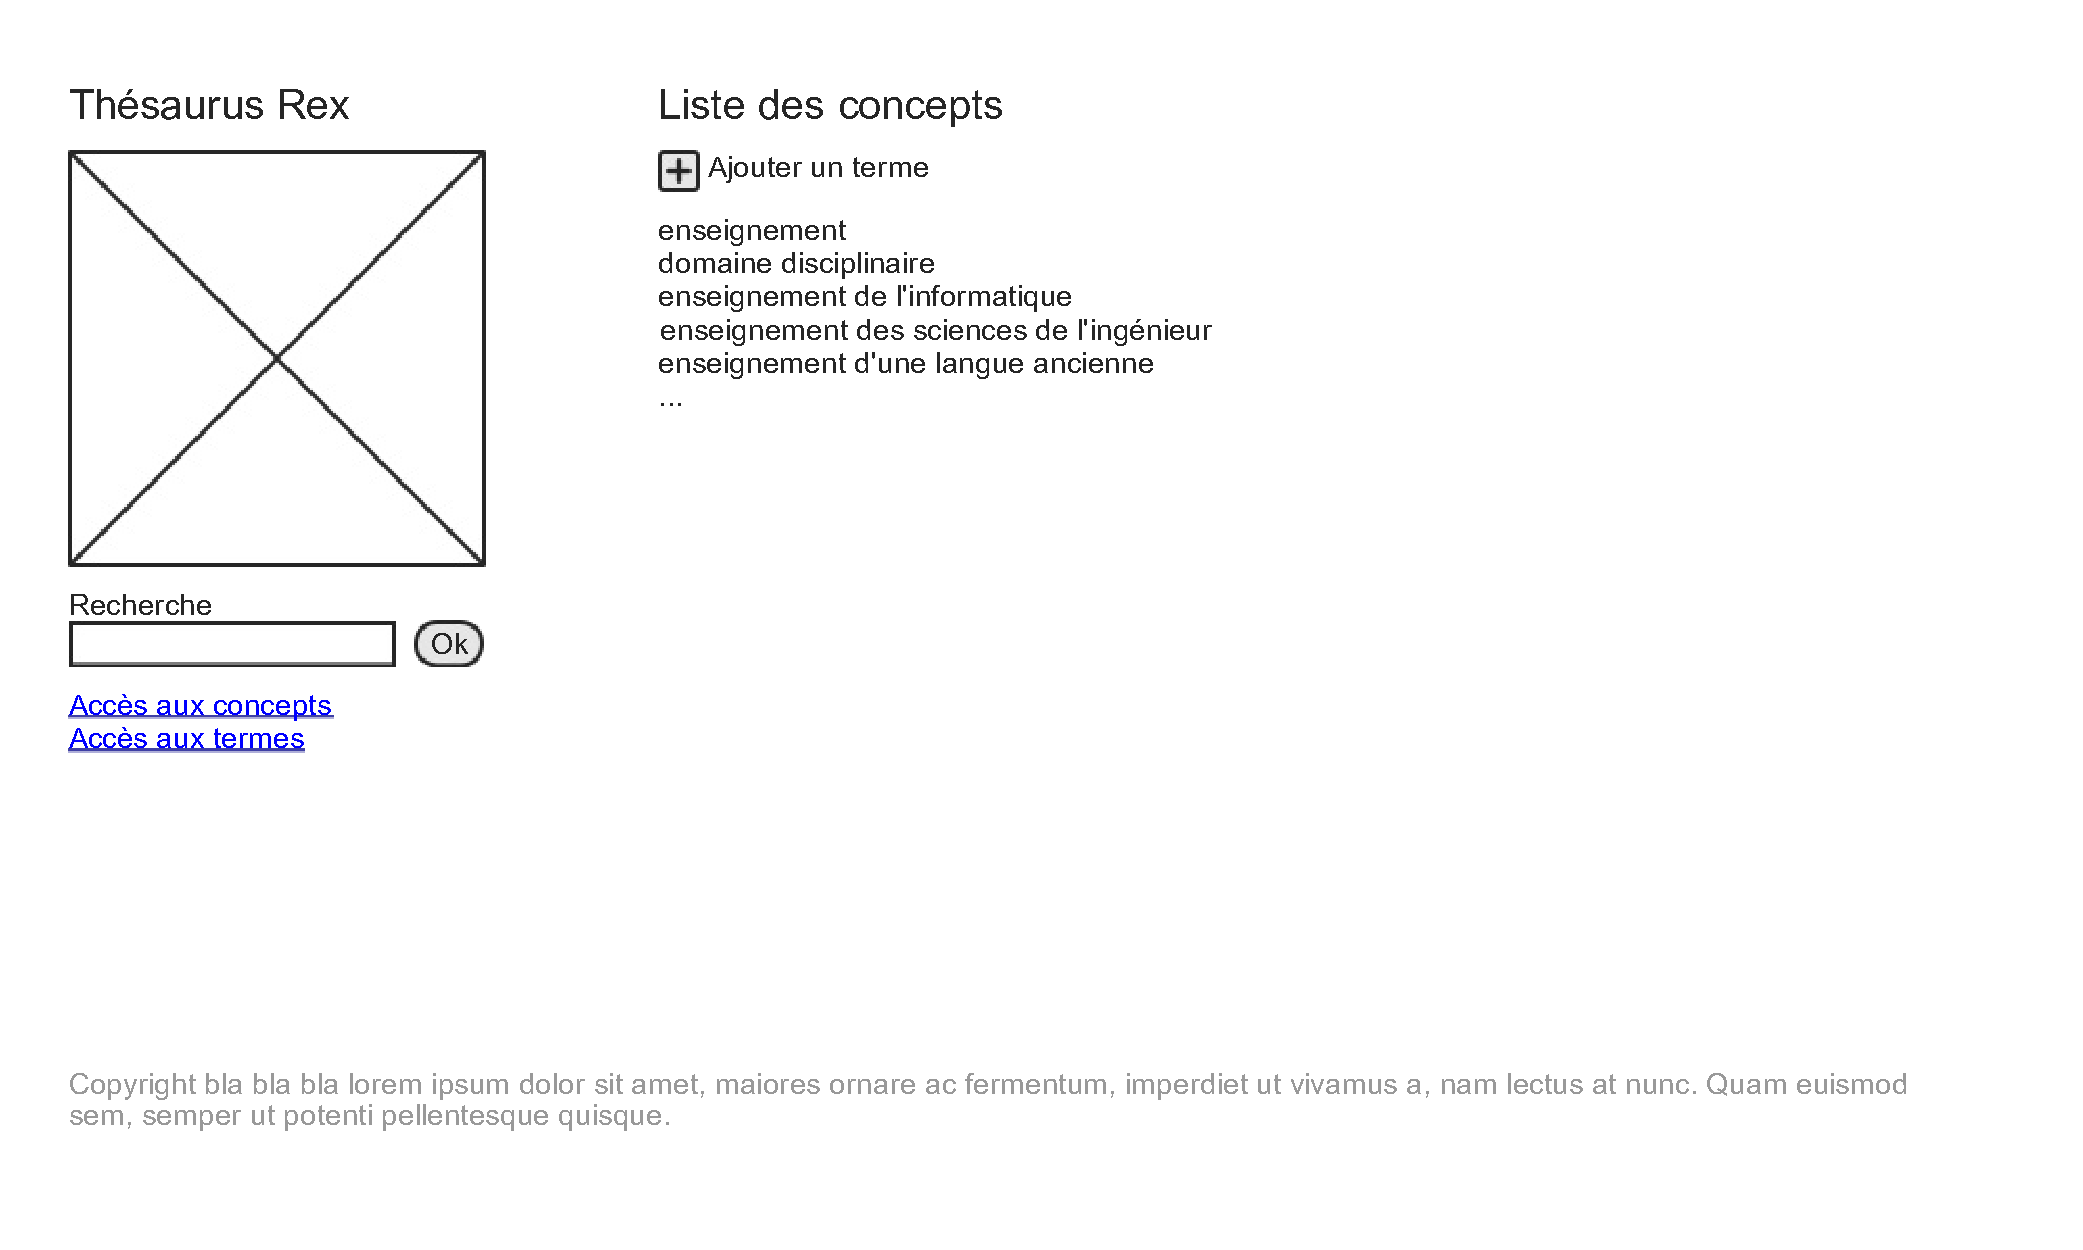
\includegraphics[width=\textwidth]{files/template_termes}
\end{center}
\caption{Template de visualisation des termes.}
\end{figure}

\subsubsection{Édition d'un terme}

Lors du clique sur un terme dans la liste, le formulaire d'édition suivant apparaît.
\begin{figure}[H]
\begin{center}
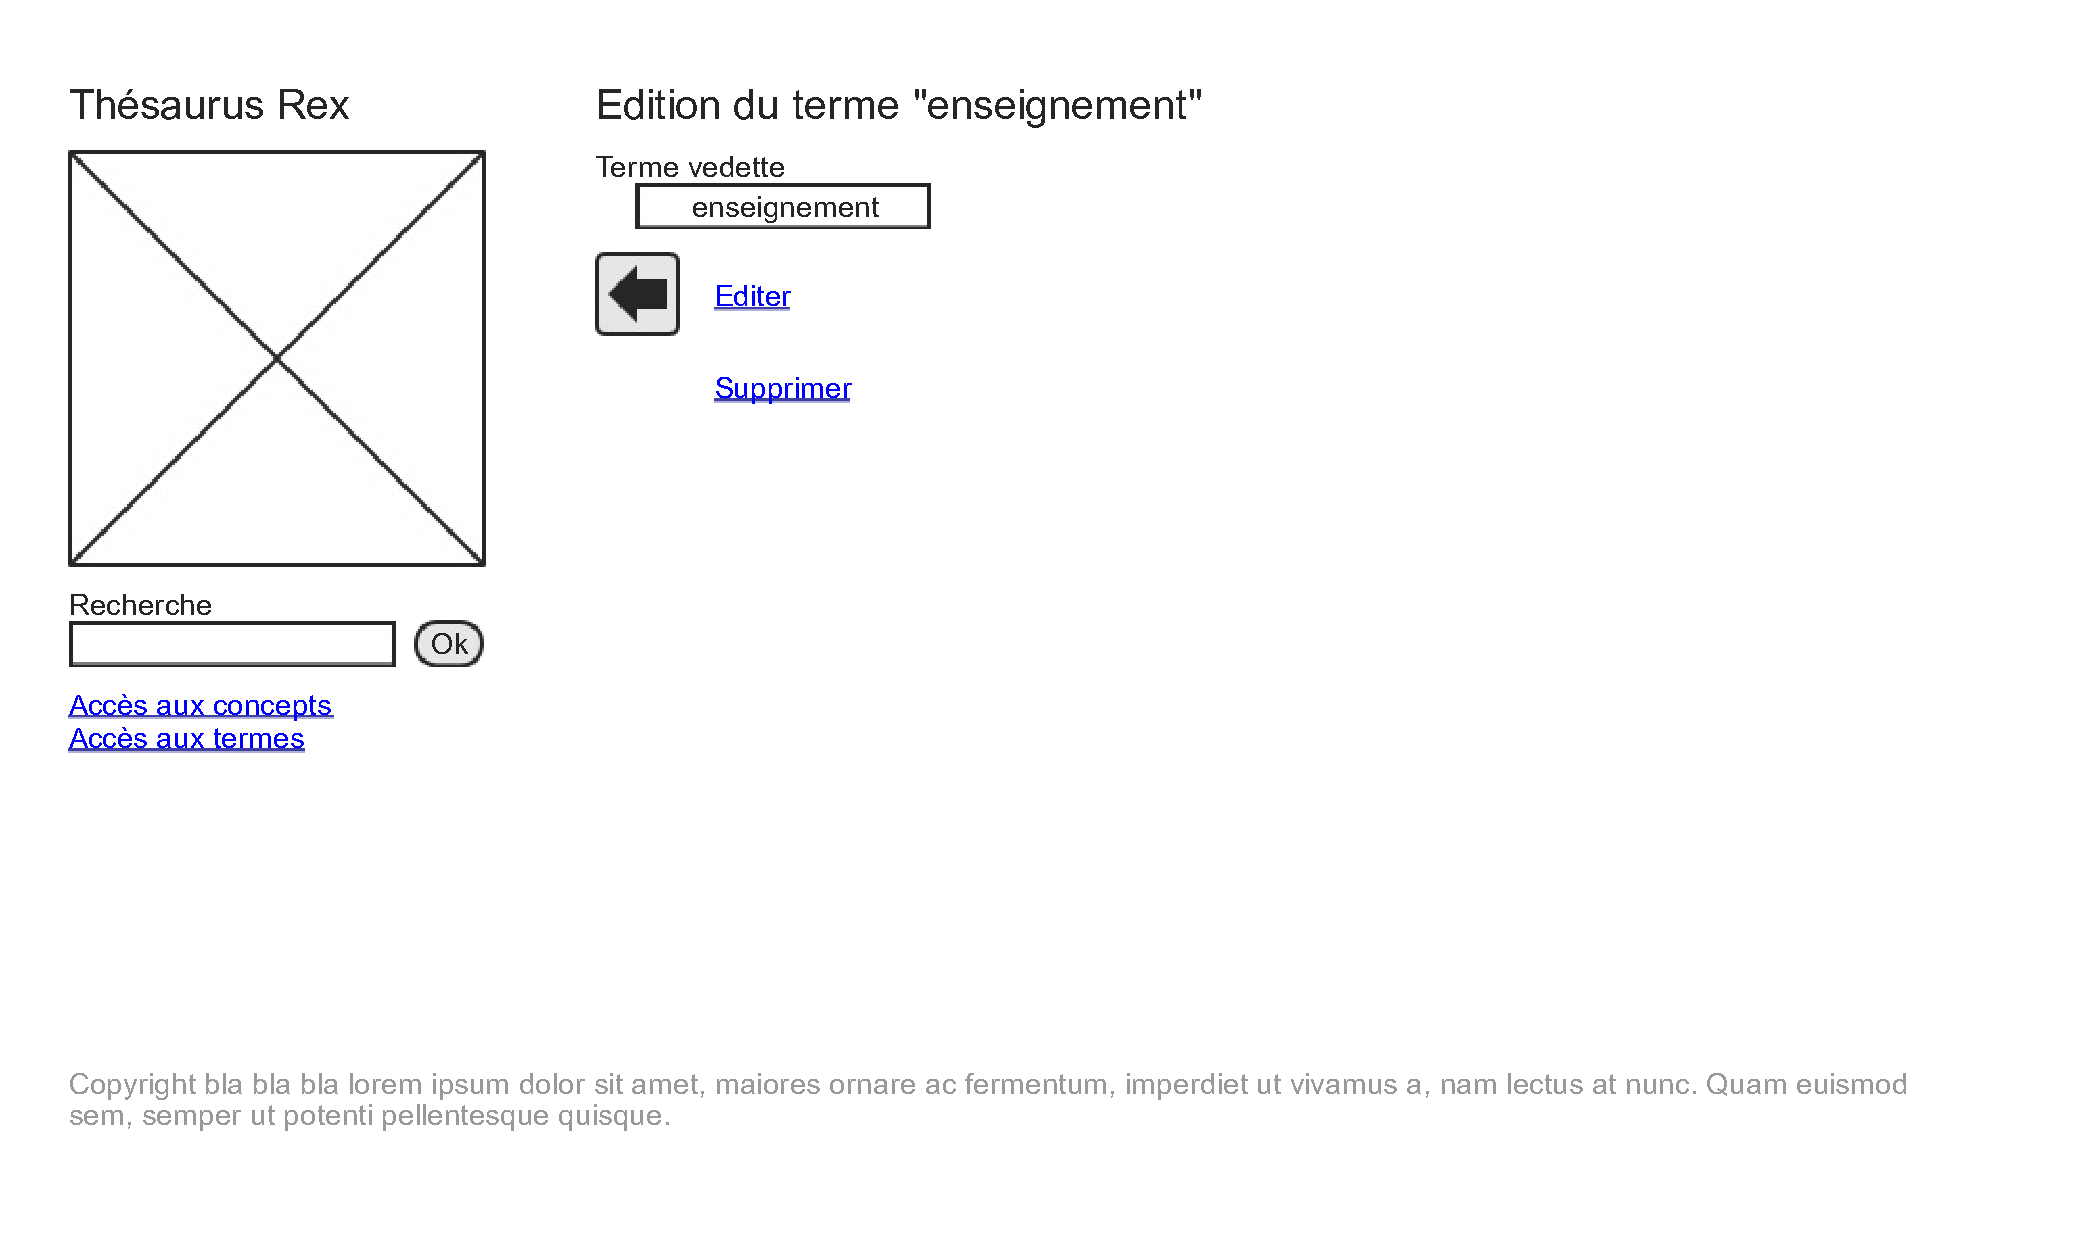
\includegraphics[width=\textwidth]{files/template_terme_edit}
\end{center}
\caption{Template du formulaire d'ajout d'un concept.}
\end{figure}
